\documentclass[a4paper,rep]{thesisby}

\usepackage[utf8]{inputenc}
\usepackage[english, russian]{babel}
\usepackage[hidelinks]{hyperref}
\hypersetup{
    allcolors=black
}

\usepackage{lastpage} % для указания общего числа страниц
\usepackage{amsmath} % для математических формул
\usepackage{IEEEtrantools} % для создания многострочных математических формул
\usepackage{commath} % для знака модуля

% для подсчёта числа источников литературы,
% но работает только после второй сборки
\usepackage{totcount}
\newtotcounter{citenum}
\def\oldcite{}
\let\oldcite=\bibcite
\def\bibcite{\stepcounter{citenum}\oldcite}

\newcommand{\No}{\textnumero}

\begin{document}

\include{parts/titlepage}
\clearpage

\chapter*{РЕФЕРАТ}

% регистрируем счётчики в системе totcounter
\regtotcounter{totalcount@figure}
\regtotcounter{totalcount@table}       % Если поставить в преамбуле то ошибка в числе таблиц
\regtotcounter{TotPages}               % Если поставить в преамбуле то ошибка в числе страниц
\regtotcounter{citenum}

Отчёт \formbytotal{TotPages}{страниц}{а}{ы}{},
1 часть,
\formbytotal{totalcount@figure}{рисун}{ок}{ка}{ков},
\formbytotal{totalcount@table}{таблиц}{а}{ы}{}.
\formbytotal{citenum}{источник}{}{а}{ов}.
\bigskip

Ключевые слова:
МЕТОД ПОЛНОСТЬЮ ПАРАЛЛЕЛЬНОЙ РАЗНОСТНОЙ ЭВОЛЮЦИИ,
ИНТЕРПРЕТАТОР ЯЗЫКА R,
МЕЖПРОЦЕССОРНОЕ ВЗАИМОДЕЙСТВИЕ,
СИНХРОНИЗАЦИЯ ОБРАБОТКИ ДАННЫХ.

Целью работы является развитие
метода ППРЭ,
улучшение взаимодействия между методом оптимизации
и функционалом качества.

Учитывая, что для решения задачи
минимизации произвольной целевой функции
не существует универсального алгоритма,
разработка и усовершенствование
методов их решения остаётся актуальной задачей.

В данной работе был спроектирован
способ увеличения производительности
метода разностной эволюции
для поиска параметров математических моделей.
Была получена реализация
с применением распараллеливания вычислений
благодаря увеличению числа интерпретаторов.
Проведено тестирование быстродействия
новой реализации и показана эффективность улучшения.


\clearpage

\tableofcontents
\clearpage

\chapter*{ОБОЗНАЧЕНИЯ И СОКРАЩЕНИЯ}
\addcontentsline{toc}{section}{ОБОЗНАЧЕНИЯ И СОКРАЩЕНИЯ}

\textbf{РЭ} --- разностная эволюция (Differential Evolution);

\textbf{DEEP, ППРЭ} --- полностью параллельная разностная эволюция (Differential Evolution Entirely Parallel);

\textbf{Интерпретатор} --- программа, выполняющая пооператорный (покомандный, построчный) анализ, обработка и тут же выполнение исходной программы или запроса.


\clearpage

\chapter*{ВВЕДЕНИЕ}
\addcontentsline{toc}{section}{ВВЕДЕНИЕ}

Проведение вычислительного эксперимента
в большинстве случаев обходится значительно дешевле,
чем проведение соответствующего эксперимента
над реальным биологическим объектом.
Именно поэтому важно развивать новые подходы в моделировании.

Важным классом программ для моделирования
являются пакеты программ
для решения обратной задачи математического моделирования.
Постановка задачи ставится
как минимизация функционала качества
при условии ограничений на параметры.

Для обратной задачи чаще всего модель известна,
но не известны некоторые параметры модели.
Задача заключается в нахождение этих параметров,
например, из данных уже проведённых экспериментов,
либо постановки дополнительных экспериментов,
называемых активным наблюдением.

Методы оптимизации можно классифицировать
в соответствии с задачами оптимизации
на локальные методы,
которые сходятся к локальному экстремуму целевой функции
(в случае унимодальной функции,
экстремум единственный и одновременно
является глобальным экстремумом)
и глобальные методы,
которые стремятся к выявлению
глобальных тенденций поведения целевой функции
и поиску глобального экстремума.

Метод полностью параллельной разностной эволюции
(далее ППРЭ, DEEP) \cite{Kozlov11, Kozlov13}
является модификацией стохастического метода оптимизации,
предложенного в \cite{Storn95}.
DEEP представляет из себя эффективный метод
решения обратной задачи математического моделирования,
а именно модификация глобального стохастического метода
и метод оптимального наискорейшего спуска
для поиска минимума функционала качества
на основе необходимого условия стационарности первого порядка.
Это значит, что он способен недетерминированно
(т.е. с использованием вероятностных методов)
находить экстремум для многоэкстремальных целевых функций
только с использованием вычисления целевой функции
в точках приближения без требования вычисления частных производных функции.

Целью работы является развитие метода ППРЭ,
улучшение взаимодействия между
методом оптимизации и функционалом качества,
что приводит к увеличению производительности.

Математические модели в биоинформатике
в большинстве случаев создаются
в таких компьютерных системах расчетов
как R, MATLAB, Octave и других.
Нахождение параметров в таких моделях
требует многократного вычисления решений,
что влечет большие накладные расходы на запуск
того или иного интерпретатора.
Однако, интерпретатор может быть встроен в программу ППРЭ,
что позволит запускать нужное число копий один раз,
и, тем самым сократить время вычислений, для некоторых задач в разы.

Таким образом,
развитие методов решения обратной задачи математического моделирования
и эффективное распараллеливание существующих решений
является важным для исследований системной биологии.


\clearpage

\include{parts/main/header}
\section*{Теория метода DEEP}
\addcontentsline{toc}{subsection}{Теория метода DEEP}

Ниже приведено описание оригинального метода разностной эволюции
и его модификации DEEP.

Разностная эволючия (РЭ) ---
стохастический итерационный алгоритм минимизации.

Метод оперирует случайно сгенерированными векторами параметров,
называемых индивидами. 
Под вектором понимается точка n-мерного пространства
из области определения целевой функции,
которую требуется минимизировать.
Множество индивидов называется популяцией.
Одна итерация популяции РЭ называется поколением.
Первое поколение генерируется случайным образом.
Новое поколение создаётся
по заданной схеме из индивидов текущего поколения.

Идея генерации нового поколения в оригинальном алгоритме
заключается в следующем.
Для каждого индивида текущего поколения
выбираются случайным образом 3 другие индивида
из поколения и вычисляется мутантный вектор по формуле:

\begin{equation} \label{mutant}
    v = v_1 + S \cdot (v_2 - v_3),
\end{equation}

где \begin{math}S\end{math} некоторая положительная константа масштабирования.

Производится операция скрещивания мутантного вектора с исходным,
замещением некоторых координат значениями из исходного вектора.
Полученный вектор называется пробным вектором.
Если значение целевой функции на нём стало меньше,
чем было на исходном, то пробный вектор добавляется в новое поколение.
Если нет, то в новое поколение переходит исходный индивид.
Таким образом, в каждом следующем поколение новые индивиды
стремится уменьшить значение целевой функции
и при определённых условиях может быть найден глобальный минимум.

Опишем модификацию РЭ, разработанную в \cite{KozlovThesis}.

\textbf{Скрещивание с учётом значения функционала:}

Используются два мутантных вектора,
на их основе определяется третий пробный вектор.
Первый мутантный вектор определяется по соотношению \ref{mutant},
второй мутантный вектор определяется по аналогии с правилом треугольника:

\begin{IEEEeqnarray}{rCl} \label{mutant2}
    z & = & \frac{v_1 + v_2 + v_3}{3}
    + (s_2 - s_1)(v_1 - v_2) \\
    && + (s_3 - s_2)(v_2 - v_3)
    + (s_1 - s_3)(v_3 - v_1), \nonumber
\end{IEEEeqnarray}

где

\begin{equation}
    s_i = \frac{\abs{F(q_i)}}
    {\abs{F(q_1)} + \abs{F(q_2)} + \abs{F(q_3)}},
\end{equation}

для \begin{math}i = 1, 2, 3\end{math}.

Третий пробный вектор составляется из произвольного выбора
соответствующих координат мутантных векторов.
Пробный вектор переходит в новое поколение,
если значение функционала на нём меньше.

\textbf{Полностью параллельная разностная эволюция:}

Метод РЭ имеет набор управляющих параметров,
которые влияют на скорость работы и сходимость.
К таким параметрам можно отнести
размер популяции, способ рекомбинации,
возраст старейших индивидов.

ППРЭ представляет собой модификацию метода РЭ,
поддерживающую распараллеливание
процесса вычислений.
Вычисления реализованы в несколько потоков
на многопроцессорных системах.
Каждый индивид помещается в очередь,
из которой извлекается и обрабатывается потоком.
Это позволяет существенно увеличить скорость работы.


\clearpage
\section*{Программная реализация DEEP}
\addcontentsline{toc}{subsection}{Программная реализация DEEP}
TODO


\clearpage
\section*{Использование интерпретаторов}
\addcontentsline{toc}{subsection}{Использование интерпретаторов}
TODO


\clearpage
\section*{Тестовые функции}
\addcontentsline{toc}{subsection}{Тестовые функции}

В качестве тестовой функции для минимизации
использовалась смещённая функция Растригина $R$:

\begin{equation}
    r = \sum_{i = 1}^{D}(x_i^2 - 10\cos(2 \pi x_i) + 10)
\end{equation}

\begin{equation}
    R = r\left(\frac{5.12 (x - o_r)}{100}\right) + 800
\end{equation}

Вектор параметров $x$ был выбран размера 30.

Было проведено тестирование
аналогично описанному в разделе
Численные эксперименты,
однако не были получены
статистические различия.
Отсутствие эффекта
от оптимизации может
быть объяснено тем,
что служебные функции
выполняются значительно быстрее.

\begin{center}
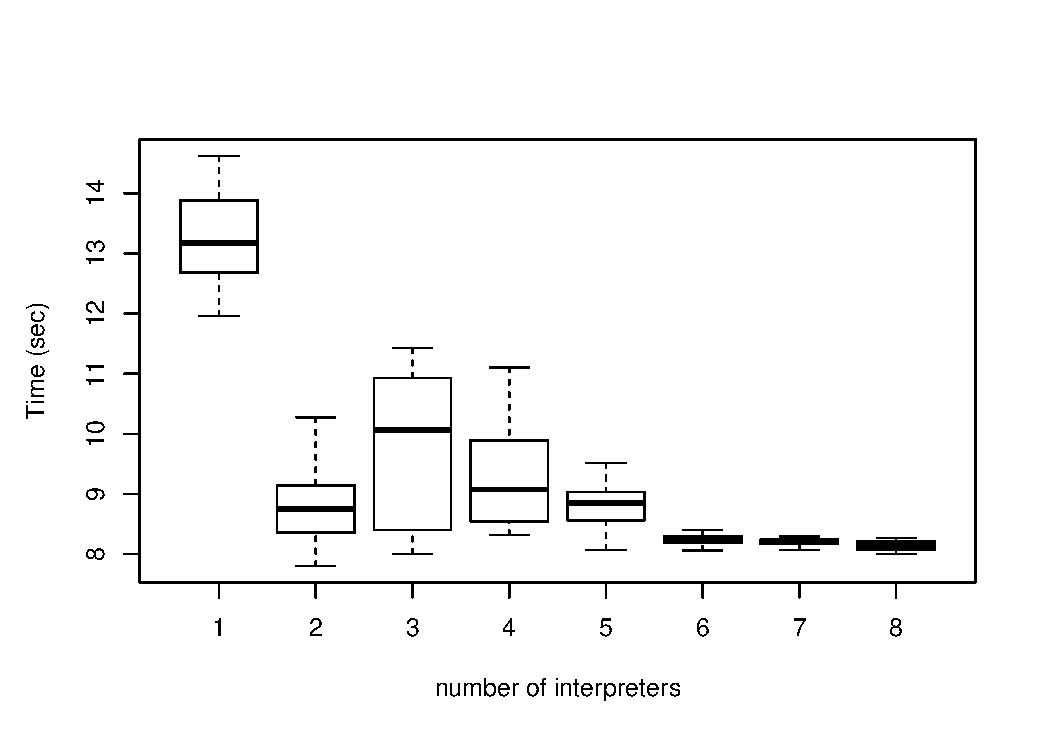
\includegraphics{rastrigin}
\end{center}

На графике видно,
что при увеличение числа интерпретаторов
время выполнения одной и той же задачи
описывает убывающую ветвь гиперболы.


\clearpage
\section*{Численные эксперименты}
\addcontentsline{toc}{subsection}{Численные эксперименты}

Тестирование проводилось на компьютере со следующими характеристиками:

\begin{tabular}{| c | c |}
    \hline
    Частота процессора & 3.7 ГГц \\ \hline
    Архитектура & 64-битная \\ \hline
    Модель процессора & Intel(R) Xeon(R) CPU E5-1620 v2 \\ \hline
    Число ядер & 8 \\ \hline
    Оперативная память & 62 Гб \\ \hline
    Объём жесткого диска & 300 Гб \\
    \hline
\end{tabular}

Старой реализацией будем называть
изначальную реализацию,
где для вычисления функционала
на векторе параметров запускался
новый интерпретатор и
заного происходила загрузка
функции скрипта.

Новым вариантом реализации
будем называть реализацию,
где используется очередь задач
и пул потоков,
интерпретаторы инициализируются
один раз и не подвергаются перезапуску,
то есть время жизни интерпретатора
завершается с окончанием
вычислений функционала.

План тестирования заключался
в сравнение времени работы
старой и новой реализаций
при одинаковых параметрах.
Проводились многократные запуски
с целью подтверждения или опровержения
гипотезы о статистической значимости различий
времени работы реализаций.
Под нулевой гипотезой будет пониматься
различие метематического ожидания
старой и новой реализаций.

Первым этапом численного эксперимента
было получение замеров времени
работы приложения
при различных комбинациях параметров.

Параметрами были выбраны следующие характеристики:

\begin{itemize}
    \item \textbf{Число потоков (\textit{i})}

        Для новой реализации этот параметр также
        обозначал размер пула потоков.
        Диапазон значений: 1-8.
    \item \textbf{Коэффициент размера популяции (\textit{M})}

        Размер популяции рационально выбирать
        пропорционально числу потоков,
        чтобы на каждый поток приходилась
        равная нагрузка при различном
        числе \textit{i}.

        Таким образом размер популяции равен:
        \begin{math}M * i\end{math}

        Тестирование проходило для значений:
        \begin{math}M = 5; M = 10\end{math}.
\end{itemize}

На следующих графиках представлены результаты тестирования:

% TODO

\includepdf[pages={-}]{zM10.pdf}


\clearpage
\section*{Сегментация траекторий частиц}
\addcontentsline{toc}{subsection}{Сегментация траекторий частиц}

Примером обратной задачи математического моделирования
может являться выявление параметров взаимодействий биологических молекул,
которые не могут быть измерены напрямую из экспериментов.

TODO


\clearpage

\chapter*{ВЫВОД}
\addcontentsline{toc}{section}{ВЫВОД}

Исходя из численных экспериментов
можно сделать следующие выводы:
\bigskip

\begin{enumerate}
    \item Было проведено
    успешное улучшение взаимодействия
    DEEP с использованием распараллеливания
    вычислений по интерпретаторам.
    Реализованная интеграция сохраняет
    кроссплатформенность DEEP,
    так как в основе решения
    использовалась библиотека GLib,
    легко портируемая на разные
    операционные системы без
    больших изменений.

    \item Для задачи
    сегментации траекторий частиц
    был достигнут четырёхкратный
    прирост производительности
    на четырёх параллельных потоках
    с четырьмя интерпретаторами
    по сравнению со старой реализацией.
\end{enumerate}


\clearpage

\chapter*{ЗАКЛЮЧЕНИЕ}
\addcontentsline{toc}{section}{ЗАКЛЮЧЕНИЕ}

Целью работы было развитие метода ППРЭ,
путём улучшения интеграции
между методом оптимизации
и функционалом качества.
В результате исследования
предполагалось увеличить
эффективность реализованной
модификации метода ППРЭ
путём встраивания интерпретаторов
и экономии процессорного времени
на их инициализацию.

ППРЭ является методом
полностью параллельной разностной эволюции,
который используется для решения
обратной задачи математического моделирования.

Показана эффективность
оптимизации в сравнении с
прошлой реализацией.
Модификация ППРЭ
была разработана на основе
открытой кроссплатформенной
библиотеки GLib.

Полученная реализация
была протестирована на
прикладной задаче
сегментации траекторий частиц.
ППРЭ использовалась в этой задаче
для нахождения вероятностей переходов и
параметров движений
скрытой марковской модели по
экспериментальным данным.
В качестве тестовой функции
также использовалась
смещённая функция Растригина.

Работа развивает метод deep
в направлении улучшения интеграции,
что ведёт к увеличению количества
проверяемых гипотез.


\clearpage

\bibliographystyle{utf8gost71u}
\bibliography{citations}

\end{document}

